At tree--level, there are three contributions to the $W^+W^+$ production in association with two jets: the pure EW component $\mathcal{O}(\alpha_{ew}^6)$, the QCD background $\mathcal{O}(\alpha_s^2\alpha_{ew}^4)$ and the interference $\mathcal{O}(\alpha_s\alpha_{ew}^5)$.\\
Concerning the QCD contribution, it is worth noticing that for quantum numbers conservation external gluons cannot contribute at LO, thus the $\mathcal{O}(\alpha_s^2\alpha_{ew}^4)$ diagrams only involve $t/u$--channel virtual gluons.\\

The three contributions to the the jet--jet invariant mass $M_{jj}$ and positive rapidity difference $|\Delta y_{jj}|$ distributions are shown in Fig.~\ref{fig:mjjdyjj_1d}, together with their sum.
\begin{figure*}[hbt]
\centering
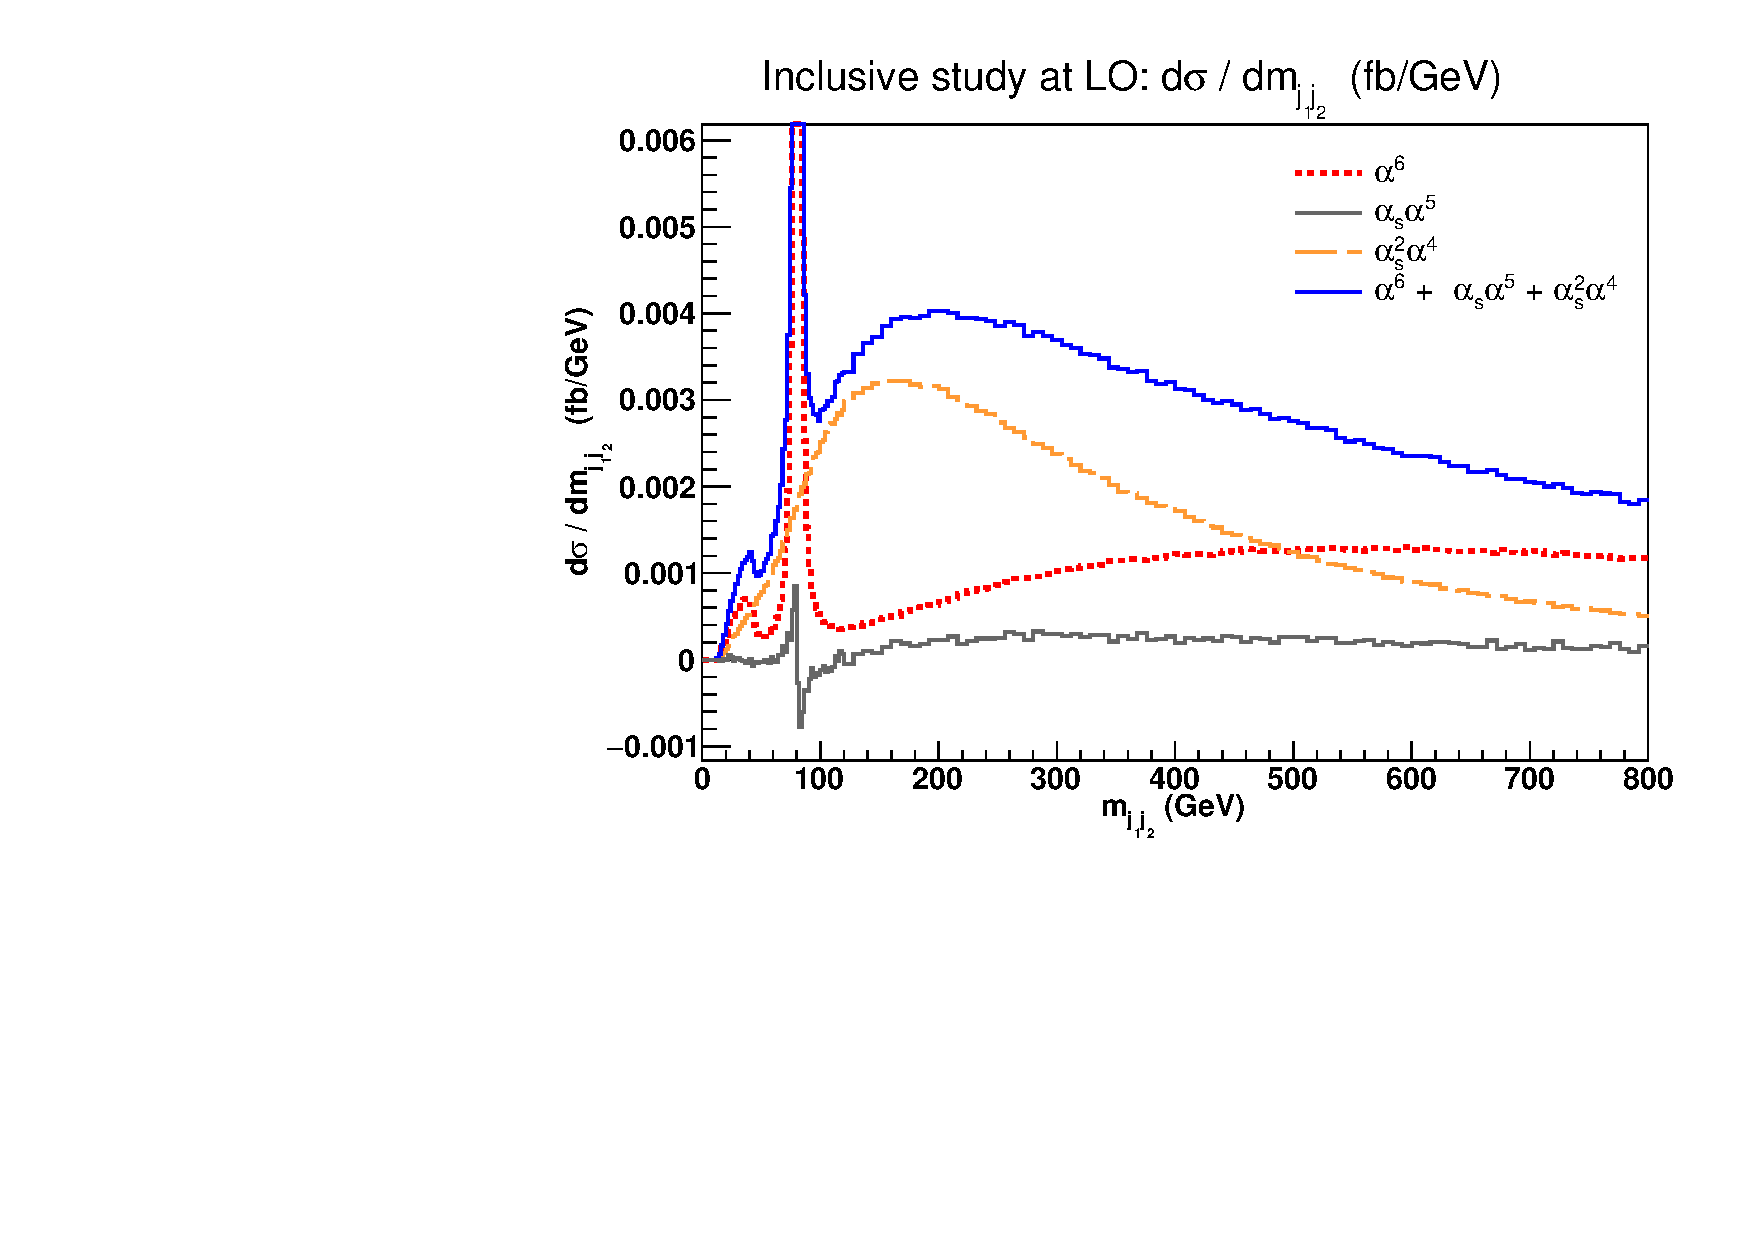
\includegraphics[scale=0.395]{figures/scanfigures/mjj_full.pdf}
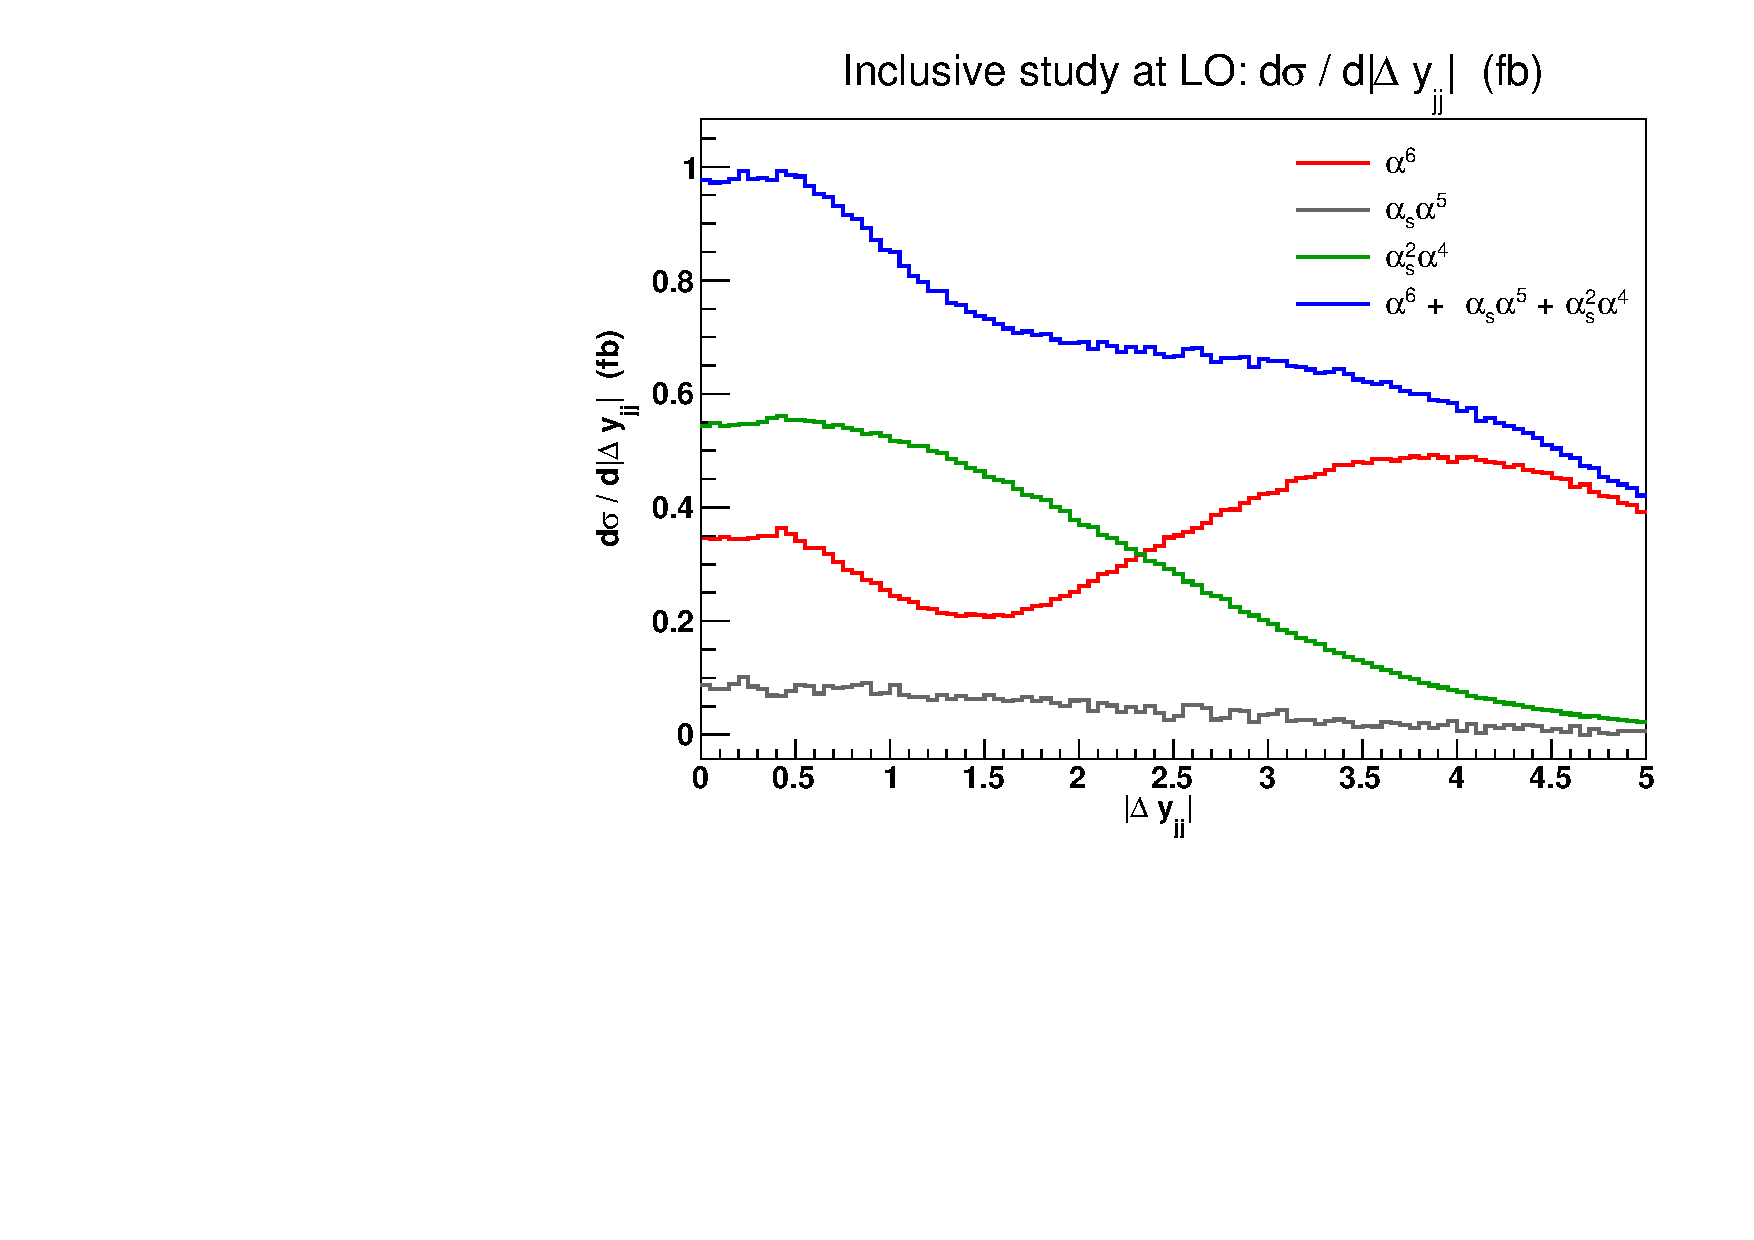
\includegraphics[scale=0.395]{figures/scanfigures/dyjj_full.pdf}
\caption{Differential distribution in the jet--jet invariant mass $M_{jj}$ (left) and the positive difference of the jet rapidities $|\Delta y_{jj}|$ (right) at LO. EW contribution in red, QCD in green, interference in gray and sum in blue. No cuts on $M_{jj}$ and $|\Delta y_{jj}|$ are applied.}
\label{fig:mjjdyjj_1d}
\end{figure*}
The interference between EW and QCD contributions is small [to be commented further]

One can also see this in three different plots in the plan $\left(m_{\Pj\Pj}, \Delta y_{\Pj\Pj}\right)$.

\begin{figure}[ht]
\centering
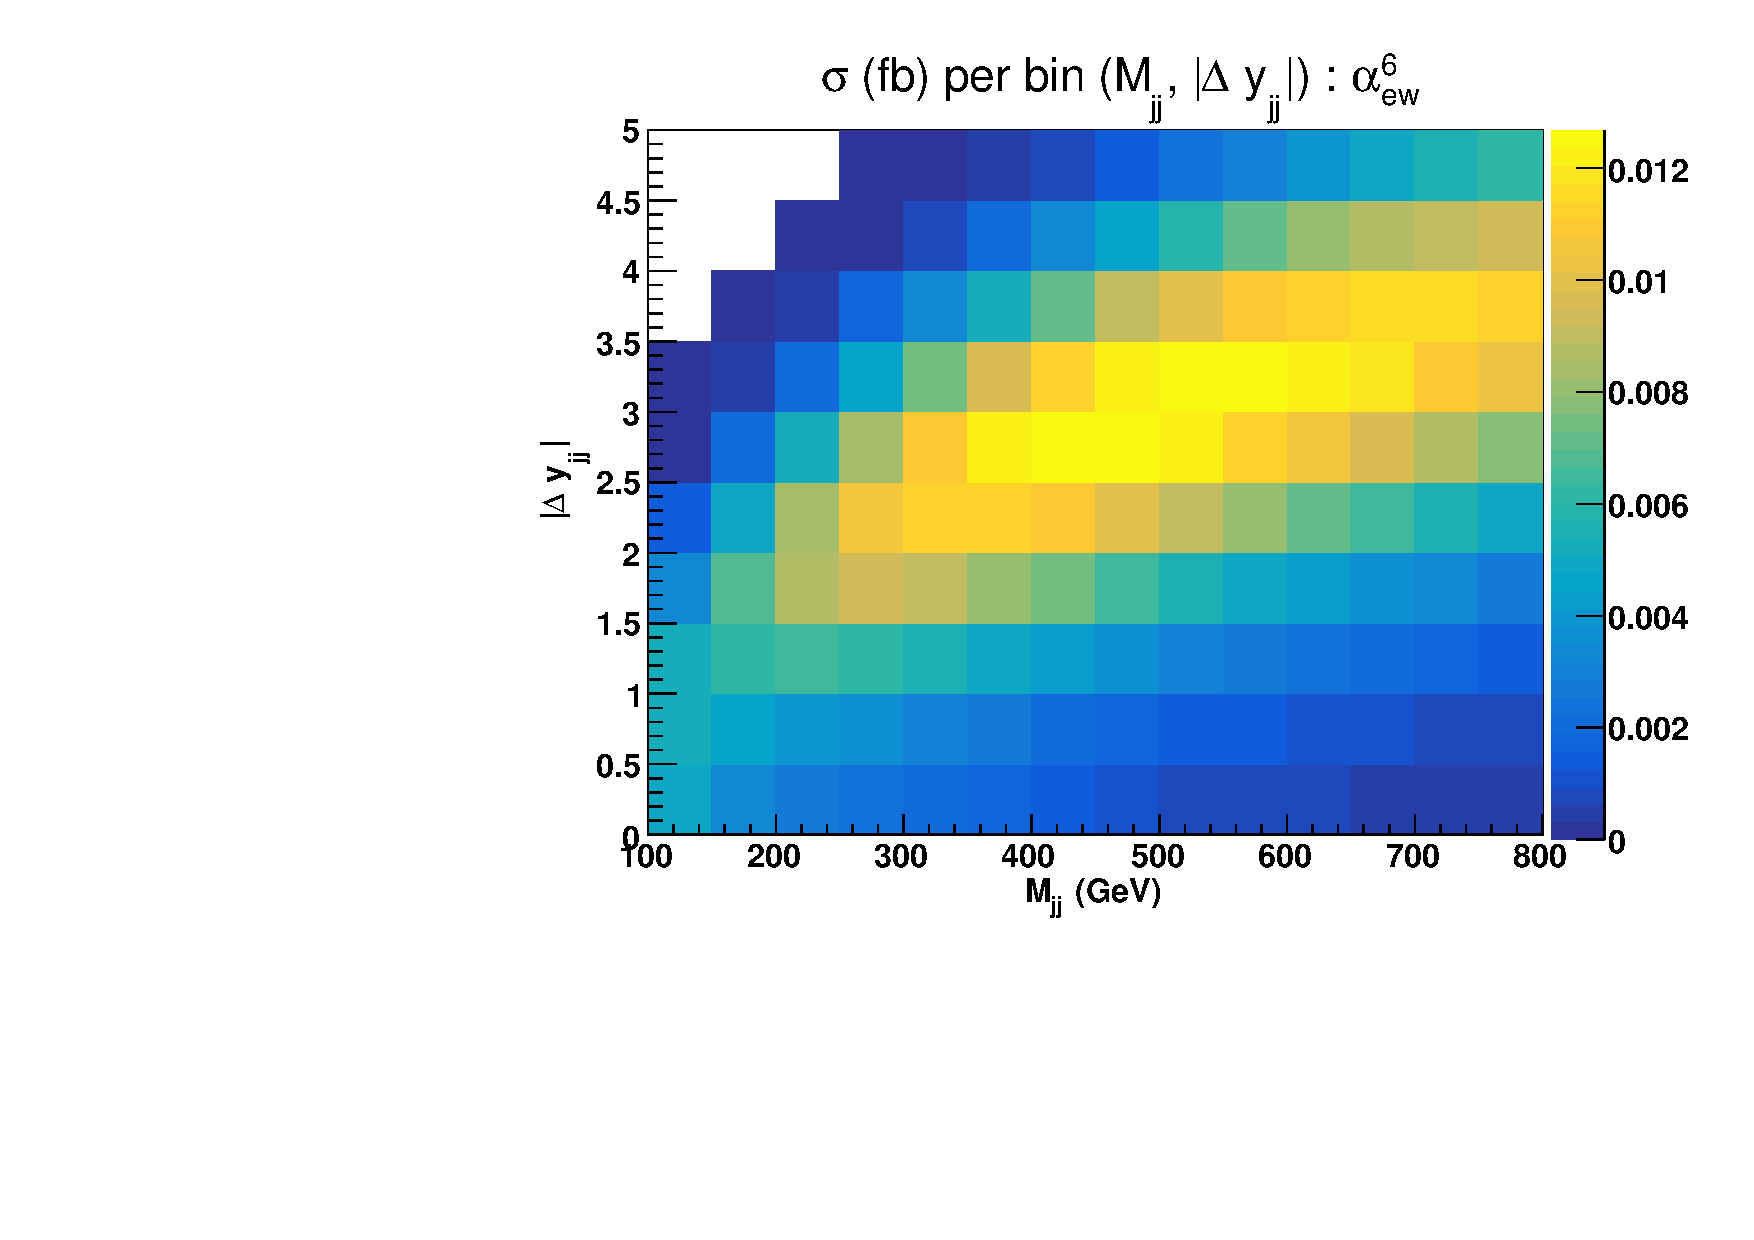
\includegraphics[scale=0.395]{figures/scanfigures/scan_ew6.pdf}
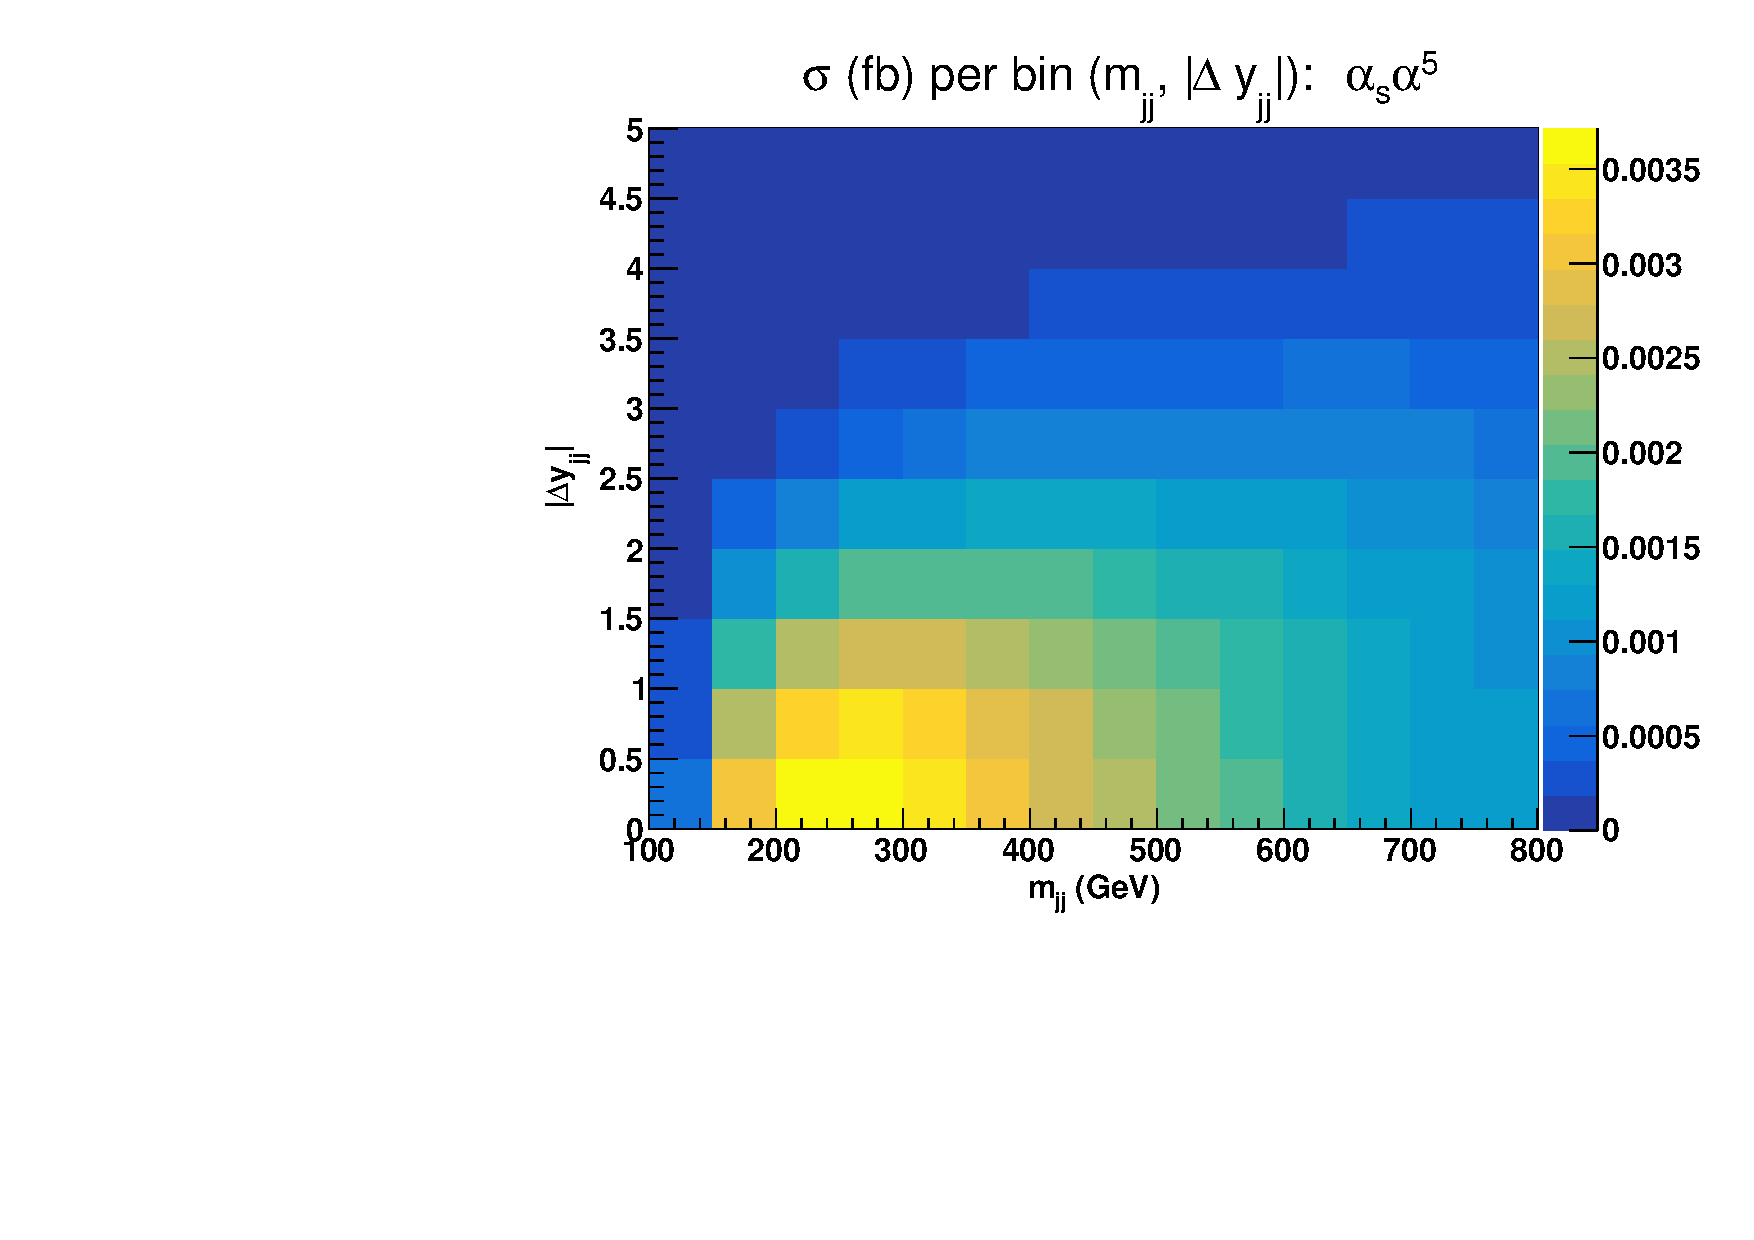
\includegraphics[scale=0.395]{figures/scanfigures/scan_ew5qcd1.pdf}
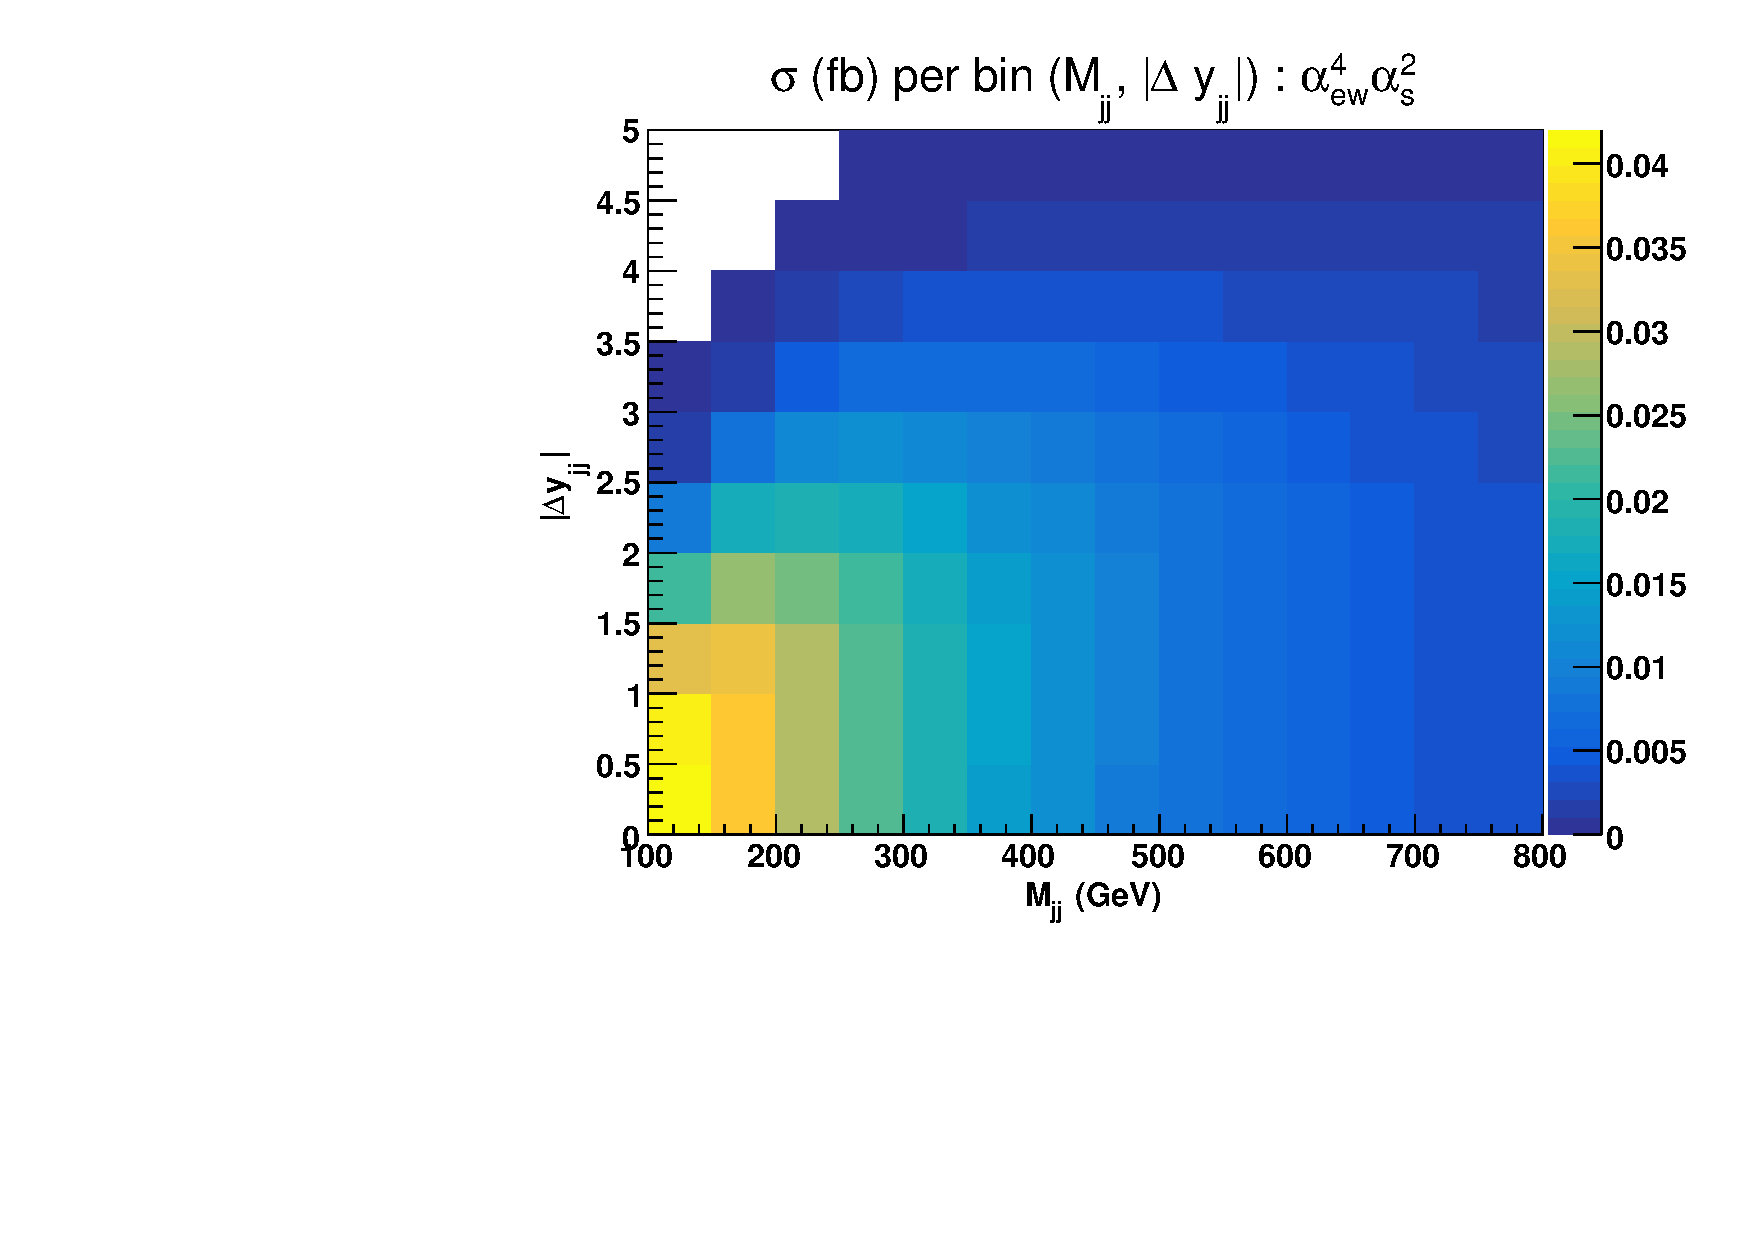
\includegraphics[scale=0.395]{figures/scanfigures/scan_ew4qcd2.pdf}
\caption{Cross sections (fb) per bin in the plan $\left(m_{\Pj\Pj}, \Delta y_{\Pj\Pj}\right)$ for the three LO contributions of orders $\mathcal{O}(\alpha^6)$ (top left), $\mathcal{O}(\alpha^5\alphas)$ (top right), and $\mathcal{O}(\alpha^4 \alphas^2)$ (bottom).}
\label{fig:mjjdyjj_2d_LO}
\end{figure}
